%% Copernicus Publications Manuscript Preparation Template for LaTeX Submissions
%% ---------------------------------
%% This template should be used for the following class files: copernicus.cls, copernicus2.cls, copernicus_discussions.cls
%% The class files, the Copernicus LaTeX Manual with detailed explanations regarding the comments
%% and some style files are bundled in the Copernicus Latex Package which can be downloaded from the different journal webpages.
%% For further assistance please contact the Publication Production Office (production@copernicus.org).
%% http://publications.copernicus.org


%% Differing commands regarding the specific class files are highlighted.


%% copernicus.cls
\documentclass[gmd]{copernicus}
\usepackage{color}
%% copernicus2.cls
%\documentclass[journal abbreviation]{copernicus2}

%% copernicus_discussions.cls
%\documentclass[journal abbreviation, hvmath, online]{copernicus_discussions}


\begin{document}

\linenumbers

\title{NCAR Model Topography Generation Software}


\author[1]{Peter Hjort Lauritzen}
\author[1]{Julio Bacmeister}
\author[1]{Patrick }

\affil[1]{1850 Table Mesa Drive, Boulder, Colorado, USA}
\affil[2]{ADDRESS}

%% The [] brackets identify the author to the corresponding affiliation, 1, 2, 3, etc. should be inserted.



\runningtitle{topo}

\runningauthor{Lauritzen et al.}

\correspondence{Peter Hjort Lauritzen\\ (pel@ucar.edu)}


\received{??}
%\pubdiscuss{} %% only important for two-stage journals
%\revised{}
%\accepted{}
%\published{}

%% These dates will be inserted by the Publication Production Office during the typesetting process.


\firstpage{1}

\maketitle  %% Please note that for the copernicus2.cls this command needs to be inserted after \abstract{TEXT}



\begin{abstract}
TEXT
\end{abstract}



\introduction  %% \introduction[modified heading if necessary]
\begin{itemize}
\item topographic input data in models:
\begin{itemize}
\item resolved-scale elevation $\Phi_s$ which usually needs to be smoothed
\item $SGH$: gravity wave drag
\item anisotropic gravity wave drag (dominant sub-grid-scale orientation)
\item $SGH30$: turbulent mountain stress
\item $LANDFRAC$
\end{itemize}
\end{itemize}

\begin{itemize}
\item Should we mention dynamic topography in the CESM (Jeremy Fyke, LANL).
\end{itemize}


\section{Method}
\subsection{Continuous: separation of scales}
The separation of scales is, in continuous space, conveniently introduced using spherical harmonics. Assume that elevation (above sea level) is a smooth continuous function in which case it can be represented by a convergent expansion of spherical harmonic functions of the form
%
% (height over Sea level{\footnote{any comment on Earth not being a perfect sphere?}})
%
\begin{equation}
h(\lambda,\theta)=\sum_{m=-\infty}^\infty \sum_{n=|m|}^\infty \psi_{m,n}Y_{m,n}(\lambda,\theta),
\end{equation}
\citep[e.g.,][]{Durran} where $\lambda$ and $\theta$ are longitude and latitude, respectively, $\psi_{m,n}$ are the spherical harmonic coefficients. Each spherical harmonic function is given in terms of the associated Legendre polynomial $P_{m,n}(\theta)$:
\begin{equation}
 Y_{m,n}=P_{m,n}(\theta)e^{im\lambda}
\end{equation}
where $m$ is the zonal wavenumber and $m-|n|$ is the number of zeros between the poles and can therefore be interpreted as meridional wavenumber. 

For the separation of scales of the variance of sub-grid-scale elevation the spherical harmonic expansion is truncated at wavenumber $M$
\begin{equation}
h^{(M)}(\lambda,\theta)=\sum_{m=-M}^\infty \sum_{n=|m|}^{M} \psi^{(M)}_{m,n}Y_{m,n}(\lambda,\theta),
\end{equation}
where a triangular truncation, which provides a uniform spatial resolution over the entire sphere, is used. 

Let $h^{(tgt)}(\lambda,\theta)$ be a continuous representation of the elevation containing the spatial scales of the target grid. We do not write that in terms of spherical harmonics as the target grid may be variable resolution and therefore contains different spatial scales in different parts of the domain.

For each target grid cell $\Omega_k$, $k=1, ..,N_t$, where $N_t$ is the number of target grid cells, define the variances
\begin{eqnarray}
\text{Var}^{(tms)}_{\Omega_k}&=&\iint_{\Omega_k}\left[ h^{(M)}(\lambda,\theta)-h(\lambda,\theta)\right]^2\cos(\theta)\, d\lambda d\theta, \\
\text{Var}^{(gwd)}_{\Omega_k}&=&\iint_{\Omega_k}\left[ h^{(tgt)}(\lambda,\theta)-h^{(M)}(\lambda,\theta)\right]^2\cos(\theta)\, d\lambda d\theta.
\end{eqnarray}
So $\text{Var}^{(tms)}_{\Omega_k}$ is the variance of elevation on scales below wavenumber $M$ and $\text{Var}^{(gwd)}_{\Omega_k}$ is the variance of elevation on scales larger than wavenumber $M$ and below the target grid scale.

{\color{red}{[julio: continuous definition of dominant orientation of orography with this notation?]}}
%%%%%%%%%%%%%%%%%%%%%%%%%%%%%%%%%%%%%%%%%%%%%%%%%%%%%%%%
\subsection{Discrete}
The separation of scales is done through the use of a quasi-isotropic gnonomic cubed-grid grid in a two-step regridding procedure, that is, binning from source grid $\Lambda$ to intermediate grid $A$ (separation of scales) to target grid $\Omega$. 

\begin{figure*}[t]
\vspace*{2mm}
\begin{center}
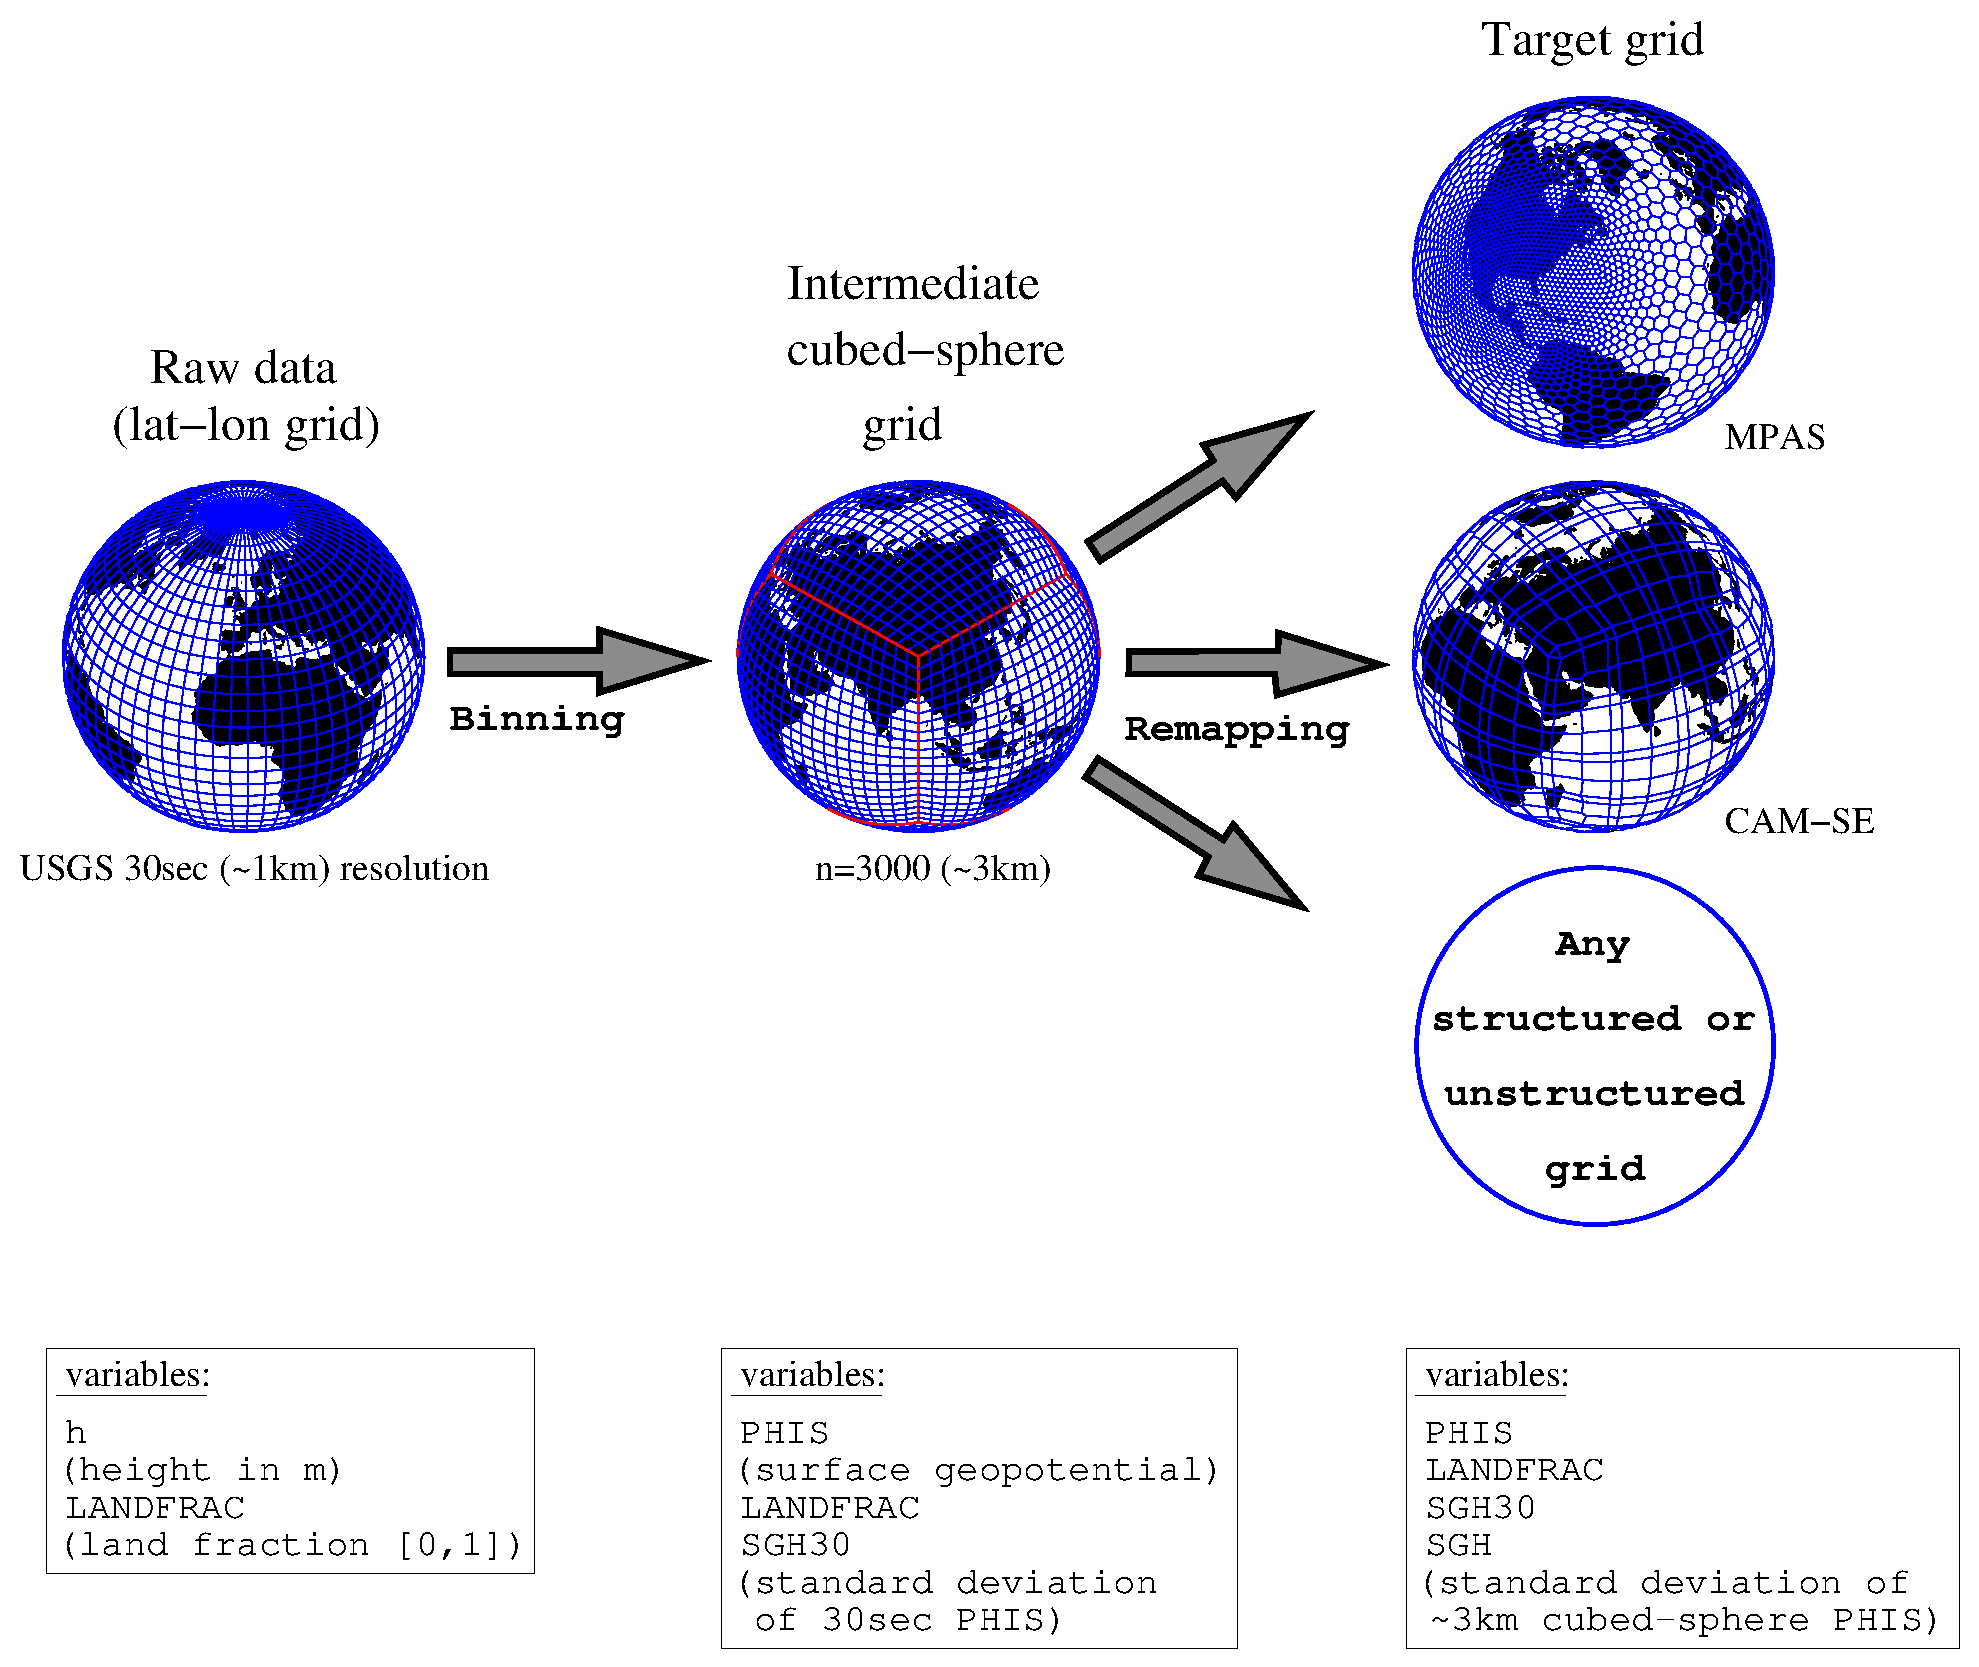
\includegraphics[width=12cm]{fig/spheres.eps}
\end{center}
  \caption{A schematic showing the regridding procedure.}\label{fig:schematic}
\end{figure*}

Any quasi-uniform spherical grid could, in theory, be used for the separation of scales. For reasons that will become clear we have chosen to use a gnomonic cubed-sphere grid resulting from an  equi-angular gnomonic (central) projection
\begin{equation}
\label{eq:GnomonicCoordinates}
x=r \, \tan \alpha \quad \mbox{and} \quad y=r \, \tan \beta; \quad
    \alpha,\beta \in \left[ -\frac{\pi}{4},\frac{\pi}{4}\right],
\end{equation}
%
% next 6 lines are copied from JCP paper - rephrase
%
\citep{RIP1996JCP} where $\alpha$ and $\beta$ are central angles in each coordinate direction, $r=R/\sqrt{3}$ and $R$ is the radius of the Earth. A point on the sphere is identified with the three-element vector $(x,y,\nu)$, where $\nu$ is the panel index. Hence the physical domain $S$ (sphere) is represented by the gnomonic (central) projection of the cubed-sphere faces, $\Omega^{(\nu)}=[-1,1]^2$, $\nu = 1,2,\dots,6$, and the non-overlapping panel domains $\Omega^{(\nu)}$ span the entire sphere: $S=\bigcup_{\nu=1}^6\Omega^{(\nu)}$. The cube  edges, however, are discontinuous. Note that any straight line on the gnomonic projection $(x,y,\nu)$  corresponds to a great-circle arc on the sphere. In the discretized scheme we let the number of cells along a coordinate axis be $N_c$ so that the total number of cells in the global domain is $6\times N_c^2$. The grid lines are separated by the same angle $\Delta \alpha=\Delta \beta=\tfrac{\pi}{2\, N_c}$ in each coordinate direction.

For notational simplicity the cubed-sphere cells are identified with one index $i$ and the relationship between $i$ and $(icube,jcube,\nu)$ is given by 
\begin{equation}
i=icube+(jcube-1)\, N_c+(\nu-1)\, N_c^2,
\end{equation}
where $(icube,jcube)\in [1,..,N_c]^2$ and $\nu \in [1,2,..,6]$. In terms of central angles the cubed-sphere grid cell $i$ is defined as
\begin{multline}
A_i= [(icube-1)\Delta \alpha-\pi/4,icube\Delta \alpha-\pi/4]\times\\
 [(jcube-1)\Delta \beta-\pi/4,jcube\Delta \beta-\pi/4],
\end{multline}
and $\Delta A_i$ denotes the spherical area. A formula for the spherical area $\Delta A_i$ of a grid cell on the gnomonical cubed-sphere grid can be found in Appendix C of \citet{LN2008MWR} (note that equation C3 is missing $\\acos$ on the right-hand side). A quasi-uniform approximately 3km resolution is obtained by using $N_c=3000$. For more details on the construction of the gnomonic grid see, e.g., \cite{LNU2010JCP}.
%
%
%
\subsubsection{Step 1: raw elevation data to intermediate cubed-sphere grid ($\Lambda \rightarrow A$)}
The `raw' elevation data is usually from a digital elevation model (DEM) such as the GTOPO30 30 arc second global dataset from the United States Geological Survey \citep[USGS][]{USGS} defined on an approximately 1km regular latitude-longitude grid. Several newer and higher resolution elevation datasets are available such as the NASA Shuttle Radar Topographic Mission (SRTM) DEM data \citep{SRTM}. The SRTM data, however, is only near-global (up to 60$^\circ$ North and South). In the remainder of this paper we assume that the raw elevation data is the USGS 30 arc second data.

The center of the regular latitude-longitude grid cells are denoted $(\lambda_{ilon},\theta_{jlat})$, $ilon=1,..., nlon$, $jlat=1, ..., nlat$. For the USGS dataset used here $nlon=43200$ and $nlat=21600$. As for the cubed-sphere we use one index $j$ to reference the grid cells
\begin{equation}
j=ilon+(jlat-1)\times nlon, \quad j\in [1, ..., N_r],
\end{equation} 
where $N_r=nlon\times nlat$. The spherical area of grid cell $\Lambda_j$ is denoted $\Delta \Lambda_j$ and the average elevation in cell $j$ is given by $\overline{h}^{(usgs)}_j$ 

This data is binned to the cubed-sphere intermediate grid by identifying in  which gnomonic cubed-sphere grid cell $(\lambda_{ilon},\theta_{jlat})$ is located. Due to the `Cartesian'-like structure of the cubed-sphere grid the search algorithm is straight forward:
\begin{itemize}
\item  use the transformation from latitude-longitude coordinates to central angle coordinates described in the Appendix of \cite{NTL2005MWRb} to compute the central angles $(\alpha, \beta)$ corresponding to the mid-point of the latitude-longitude grid cell $(\lambda_{ilon},\theta_{jlat})$.  [more details on algorithm z]
\item the indices of the cubed-sphere cell in which the center of the latitude-longitude grid cell is located is given by  
\begin{eqnarray*} 
icube &=& \verb+CEILING+\left(\frac{\alpha + \frac{\pi}{4}}{\Delta \alpha}\right),\\
jcube &=& \verb+CEILING+\left(\frac{\beta  + \frac{\pi}{4}}{\Delta \beta}\right),
\end{eqnarray*}
where the \verb+CEILING+($x$) function returns the smallest integer not less than $x$. 
\end{itemize}
The set of indices for which center points of regular latitude-longitude grid cells are located in gnomonic cubed-sphere cell $A_i$ is denoted ${\mathbb{S}}_i$. Note that since the USGS dataset is higher resolution that the cubed-sphere ${\mathbb{S}}_i$ is guaranteed to be non-empty. Through this binning process the approximate average elevation in cubed-sphere cell $i$ becomes
\begin{equation}
\overline{h}^{(cube)}_i=\frac{1}{\Delta A_i}\, \sum_{j\in {\mathbb{S}}_i}{\overline{h}}^{(usgs)}_j\Delta \Lambda_j.
\end{equation}
The binning process is straight forward since the cubed-sphere grid is essentially an equidistant Cartesian grid on each panel in terms of the central angle coordinates. This step could be replaced by rigorous remapping in terms of overlap areas between the regular latitude-longitude grid and the cubed-sphere grid using the geometrically exact algorithm of \citep{ULJ2009MWR} optimized for the regular latitude-longitude and gnomonic cubed-sphere grid pair or the more general remapping algorithm called SCRIP \citep{J1999MWR}.

The sub-grid-scale variance of elevation with respect to the cubed-sphere grid cell $i$ is
\begin{equation}
Var^{(tms)}_i=\frac{1}{\Delta A_i}\sum_{j\in {\mathbb{S}}_i} \left( \overline{h}_i^{(cube)}-{\overline{h}}^{(usgs)}_j\right)^2\, \Delta \Lambda_j.
\end{equation}

\begin{itemize}
\item mention the changes to raw data: Caspian sea, Antartica (why are these changes made?)
\end{itemize}

%
% show details of that algorithm form the code
%
%        call CubedSphereABPFromRLL(lon(i), lat(j), alpha, beta, ipanel)            
%       icube = CEILING((alpha + piq) / da)
%       jcube = CEILING((beta  + piq) / da)
%\begin{figure}[t]
%\center\includegraphics[width=35pc,angle=0]{fig/effect-of-binning}\\
%  \caption{Effect of binning (figure Curtesy of S.J. Lin (GFDL) [will be replaced with Figure from CAM data].)}\label{fig:nonconvex}
%\end{figure}
TODO: show a Figure illustrating the amount of smoothing performed by the binning!
%
\subsubsection{Step 2: cubed-sphere grid to target grid ($A\rightarrow \Omega$)}
The cell averaged values of elevation and sub-grid-scale variances ($Var^{(tms)}$ and $Var^{(gwd)}$) on the target grid are computed by rigorously remapping the variables from the cubed-sphere grid to the target grid.  The remapping is performed using CSLAM (Conservative Semi-LAgrangian Multi-tracer transport scheme) technology \citep{LNU2010JCP} that has the option for performing higher-order remapping. It s possible to use large parts of the CSLAM technology since the source grid is a gnomonic cubed-sphere grid hence instead of remapping between the gnomonic cubed-sphere grid and a deformed Lagrangian grid, as done in CSLAM transport, the remapping is from the gnomonic cubed-sphere grid to any target grid constructed from great-circle arcs (the target grid `plays the role' of the Lagrangian grid). However, a couple of modifications where made to the CSLAM search algorithm. First of all, the target grid cells can have an arbitrary number of vertices whereas the CSLAM transport search algorithm assumes that the target grid consists of quadrilaterals and the number of overlap areas are determined by the deformation of the transporting velocity field. In the case of the remapping needed in this application the target grid consists of polygons with any number of vertices and the search is not constrained by the physical relation between regular and deformed upstream quadrilaterals. Secondly, the CSLAM search algorithm for transport assumes that the target grid cells are convex which is not necessarily the case for topography target grids. The CSLAM search algorithm has been modified to support non-convex cells that are, for example, encountered in variables resolution CAM-SE (see, e.g., Fig.\ref{fig:nonconvex}); essentially that means that any target grid cell may cross a gnonomic isoline (source grid line) more than twice as is the case for transport.
%\begin{figure}[t]
%\center\includegraphics[width=15pc,angle=0]{fig/non-convex-cell/1.pdf}\\
%  \caption{Non-convex cell from variable resolution CAM-SE.}\label{fig:nonconvex}
%\end{figure}

Let the target grid consist of $N_t$ grid cells $\Omega_k$, $k=1, ..., N_t$ with associated spherical area $\Delta \Omega_k$. The search algorithm for CSLAM is used to identify overlap areas between the target grid cell $\Omega_k$ and the cubed-sphere grid cells $A_\ell$, $\ell=1,..,N_c$. Denote the overlap area between $\Omega_k$ and $A_\ell$
\begin{equation}
\Omega_{k\ell}=\Omega_k \cap A_\ell,
\end{equation}
and let $\mathbb{L}_k$ denote the set of indices for which $\Omega_k \cap A_\ell$, $\ell=1,..,N_c$, is non-empty. Then the average elevation and variance used for TMS in target grid cell $k$ are given by
\begin{eqnarray}
\overline{h}^{(targ)}_k&=&\frac{1}{\Delta \Omega_k}\sum_{\ell\in {\mathbb{L}}_k}\overline{h}^{(cube)}_\ell\, \Delta \Omega_{k\ell},\\
\overline{Var}^{(tms)}_k&=&\frac{1}{\Delta \Omega_k}\sum_{\ell\in {\mathbb{L}}_k}\overline{Var}^{(tms)}_\ell\, \Delta \Omega_{k\ell},
\end{eqnarray}
respectively. The variance of the cubed-sphere data $\overline{h}^{(cube)}$ with respect to the target grid cell average values $\overline{h}^{(targ)}$ is given by
\begin{equation}
\overline{Var}^{(sgh)}_k=\frac{1}{\Delta \Omega_k}\sum_{\ell\in {\mathbb{L}}_k}\left( \overline{h}^{(targ)}_k-\overline{h}^{(cube)}_\ell\right)^2\, \Delta \Omega_{k\ell},
\end{equation}




TEXT

\subsection{HEADING}
TEXT

\subsubsection{HEADING}
TEXT




\conclusions  %% \conclusions[modified heading if necessary]
TEXT




\appendix
\section{\\ \\ \hspace*{-7mm} Grid descriptor NetCDF file}    %% Appendix A

\subsection{asdf}                               %% Appendix A1, A2, etc.




\begin{acknowledgements}
NCAR is sponsored by the National Science Foundation (NSF). Thanks to DOE ...
\end{acknowledgements}



\bibliographystyle{copernicus}
\bibliography{bib}

%\begin{thebibliography}{}
%
%\bibitem[AUTHOR(YEAR)]{LABEL}
%REFERENCE 1
%
%\bibitem[AUTHOR(YEAR)]{LABEL}
%REFERENCE 2
%
%...
%
%\end{thebibliography}


%% Literature citations
%% command                        & example result
%% \citet{jones90}|               & Jones et al.\ (1990)
%% \citep{jones90}|               & (Jones et al., 1990)
%% \citep{jones90,jones93}|       & (Jones et al., 1990, 1993)
%% \citep[p.~32]{jones90}|        & (Jones et al., 1990, p.~32)
%% \citep[e.g.,][]{jones90}|      & (e.g., Jones et al., 1990)
%% \citep[e.g.,][p.~32]{jones90}| & (e.g., Jones et al., 1990, p.~32)
%% \citeauthor{jones90}|          & Jones et al.
%% \citeyear{jones90}|            & 1990






%% FIGURES %%%%%%%%%%%%%%%%%%%%%%%%%%%%%%%%%%%%%%%%%%%%%%%%%%%%%%%%%%%%%%%%%%%%


%% ONE-COLUMN FIGURES

%f
%\begin{figure}[t]
%\vspace*{2mm}
%\begin{center}
%\includegraphics[width=8.3cm]{FILE NAME}
%\end{center}
%\caption{TEXT}
%\end{figure}



%% TWO-COLUMN FIGURES

%f
%\begin{figure*}[t]
%\vspace*{2mm}
%\begin{center}
%\includegraphics[width=12cm]{FILE NAME}
%\end{center}
%\caption{TEXT}
%\end{figure*}


%% TABLES %%%%%%%%%%%%%%%%%%%%%%%%%%%%%%%%%%%%%%%%%%%%%%%%%%%%%%%%%%%%%%%%%%%%


%% ONE-COLUMN TABLE

%t
%\begin{table}[t]
%\caption{TEXT}
%\vskip4mm
%\centering
%\begin{tabular}{column = lcr}
%\tophline
%
%\middlehline
%
%\bottomhline
%\end{tabular}
%\end{table}


%% TWO-COLUMN TABLE

%t
%\begin{table*}[t]
%\caption{TEXT}
%\vskip4mm
%\centering
%\begin{tabular}{column = lcr}
%\tophline
%
%\middlehline
%
%\bottomhline
%\end{tabular}
%\end{table*}


%% The different columns must be seperated with a & command and should
%% end with \\ to identify the column brake.

%%%%%%%%%%%%%%%%%%%%%%%%%%%%%%%%%%%%%%%%%%%%%%%%%%%%%%%%%%%%%%%%%%%%%%%%%%%%%%


%% If figures and tables must be numbered 1a, 1b, etc. the following command
%% should be inserted before the begin{} command.

%\addtocounter{figure}{-1}\renewcommand{\thefigure}{\arabic{figure}a}


\end{document}
